\documentclass[a4paper]{report}

%====================== PACKAGES ======================

\usepackage[french]{babel}
\usepackage[utf8x]{inputenc}
%pour gérer les positionnement d'images
\usepackage{float}
\usepackage{amsmath}
\usepackage{graphicx}
\usepackage[colorinlistoftodos]{todonotes}
\usepackage{url}
%pour les informations sur un document compilé en PDF et les liens externes / internes
\usepackage{hyperref}
%pour la mise en page des tableaux
\usepackage{array}
\usepackage{tabularx}
%pour utiliser \floatbarrier
%\usepackage{placeins}
%\usepackage{floatrow}
%espacement entre les lignes
\usepackage{setspace}
%modifier la mise en page de l'abstract
\usepackage{abstract}
%police et mise en page (marges) du document
\usepackage[T1]{fontenc}
\usepackage[top=2cm, bottom=2cm, left=2cm, right=2cm]{geometry}
%Pour les galerie d'images
\usepackage{subfig}

%====================== INFORMATION ET REGLES ======================

%rajouter les numérotation pour les \paragraphe et \subparagraphe
\setcounter{secnumdepth}{4}
\setcounter{tocdepth}{4}

\hypersetup{							% Information sur le document
pdfauthor = {Premier Auteur,
			Deuxième Auteur,
			Troisième Auteur,
    		Quatrième Auteur,
            Cinquième Auteur,
            Sixième Auteur},			% Auteurs
pdftitle = {Sharelet -
			Rapport Sprint 1},			% Titre du document
pdfsubject = {Mémoire de Projet},		% Sujet
pdfkeywords = {Tag1, Tag2, Tag3, ...},	% Mots-clefs
pdfstartview={FitH}}					% ajuste la page à la largueur de l'écran
%pdfcreator = {MikTeX},% Logiciel qui a crée le document
%pdfproducer = {}} % Société avec produit le logiciel

%======================== DEBUT DU DOCUMENT ========================

\begin{document}

%régler l'espacement entre les lignes
\newcommand{\HRule}{\rule{\linewidth}{0.5mm}}

%page de garde
\begin{titlepage}
\begin{center}

% Upper part of the page. The '~' is needed because only works if a paragraph has started.

\includegraphics[width=0.6\textwidth]{images/logo-ephec}\\[1cm]
{\large 3TI - 2017-2018}\\[0.5cm]

{\large T3042 - Projet d'intégration}\\[0.8cm]

% Title
\HRule \\[0.7cm]
{ 

\includegraphics[width=0.5\textwidth]{images/sharelet.png}\\
}
{\huge \bfseries Sprint 1\\[0.75cm] }
{\bfseries Groupe N°1744002 }\\[1cm]
\HRule \\[2.5cm]

% Author and supervisor
\begin{minipage}{0.4\textwidth}
\begin{flushleft} \large
\emph{Auteurs:}\\
\textsc{Brancart} Clément\\
\textsc{Courtin} Amélie\\
\textsc{Delfosse} Danielle\\
\textsc{Mbarushimana} Nadia\\
\textsc{Pettens} Denis\\
\textsc{Surleraux} Nicolas\\
\end{flushleft}
\end{minipage}
\begin{minipage}{0.4\textwidth}
\begin{flushright} \large
\emph{Professeurs Encadrants:} \\
\textsc{Vroman} Marie-Noël \\
\textsc{Van Den Schrieck} Virginie \\
\end{flushright}
\end{minipage}

\vfill

% Bottom of the page
{\large \today}

\end{center}
\end{titlepage}

%page blanche
%\newpage
%~

%ne pas numéroter cette page
%\thispagestyle{empty}
%\newpage

%\tableofcontents
%\thispagestyle{empty}
%\setcounter{page}{0}
%ne pas numéroter le sommaire

%\newpage

%espacement entre les lignes d'un tableau
\renewcommand{\arraystretch}{1.5}

%====================== INCLUSION DES PARTIES ======================

%~
%\thispagestyle{empty}
%recommencer la numérotation des pages à "1"
%\setcounter{page}{0}
%\newpage
\chapter{Review et retrospective du premier sprint}

\section{Récapitulatif du projet}

Dans le cadre du cours de projet d'intégration, nous avons été amenés à choisir un produit à la fois innovant et représentatif de nos compétences acquises au cours des 3 dernières années. Ce produit doit répondre à la problématique posée par la  \textit{Maison du Développement Durable} de Louvain-la-neuve qui est la suivante : 
\begin{center}
\textbf{Comment réduire l'émission de CO² ?}
\end{center}

Après pas mal de discussions, nous avons décidé de viser la consommation électrique. En effet, il existe beaucoup trop de consommation électrique superficielle et nous voulions remédier à ce problème. \\


Notre produit, \textbf{Sharelet}, est une prise connectée. Elle communiquera avec une interface web, permettant une surveillance de la consommation et un contrôle distant de la prise. Les données seront centralisées, permettant une comparaison avec les autres utilisateurs!  \\ 

Avec les données, nous voudrions comparer et réaliser des statistiques pour que les cilents puissent se situer quant à leur consommation par rapport à d'autres. 

Nous souhaitons également avoir une communauté non silencieuse qui partagerait trucs et astuces pour consommer de manière plus raisonnable. 

\newpage
\section{Avancement dans les Users Stories}
Voici les Users Stories implémenter dans ce sprint. Elles ne sont pas toutes à 100\% finies dûes aux problématiques rencontrées.\\
Il y a un total de 20 points pour ce sprint. \\
\begin{center}
    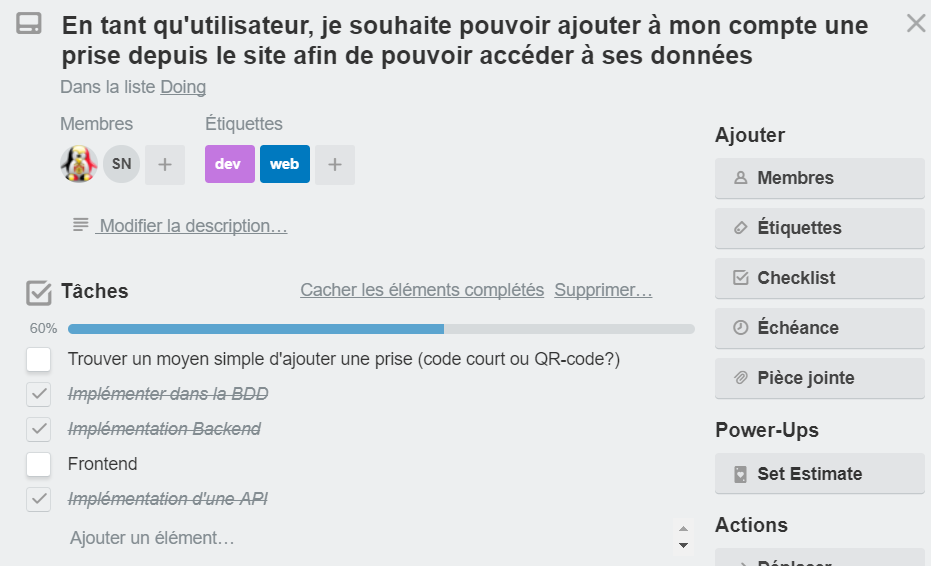
\includegraphics[width=0.8\textwidth]{images/US01.png}~\\[0.5cm]
 \end{center}
 \begin{flushright}
    Cette US a été mise à 5 points \\
 \end{flushright}
\begin{center}
    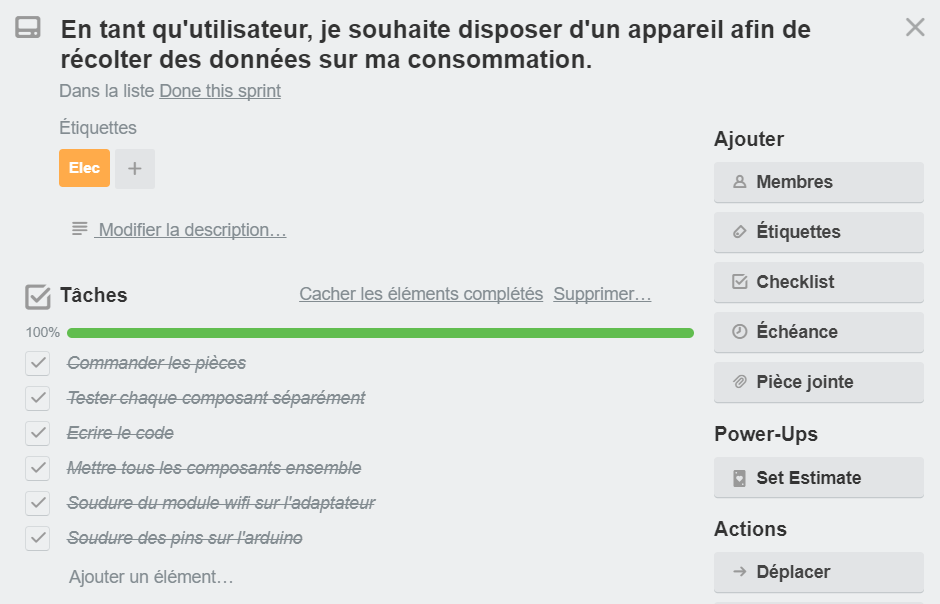
\includegraphics[width=0.8\textwidth]{images/US02.png}~\\[0.5cm]
 \end{center}
 \begin{flushright}
    Cette US a été mise à 15 points \\ 
\end{flushright}
\begin{center}
    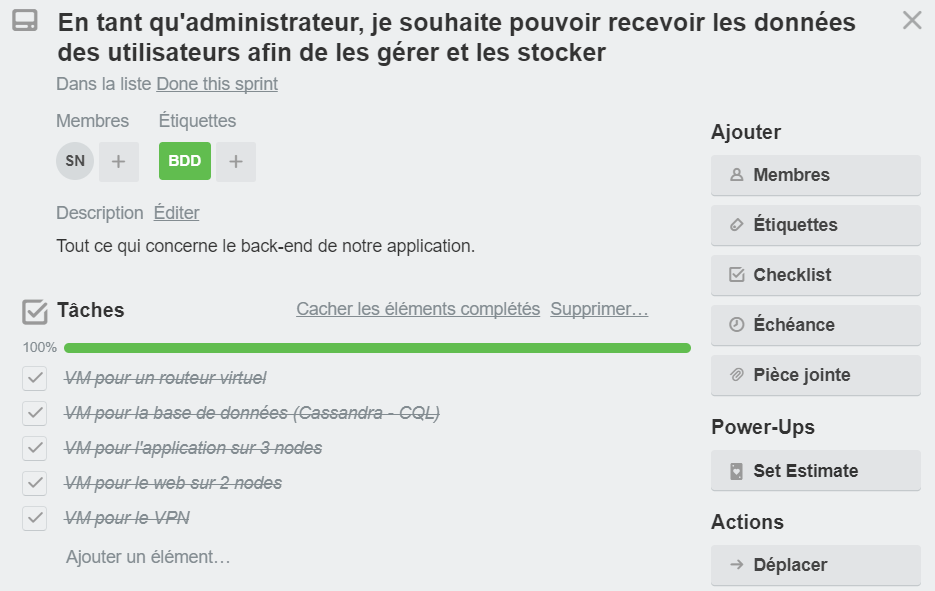
\includegraphics[width=0.8\textwidth]{images/US03.png}~\\[0.5cm]
     \end{center}
\begin{flushright}
 Cette US a été mise à 5 points \\ 
\end{flushright}

\section{Estimation de la vélocité de l'équipe}
\begin{tabularx}{15cm}{|c|p{4.5cm}|X|}
    \hline
    \textbf{Catégorie} & \textbf{Membres} & \textbf{Remarques} \\
    \hline
    Electronique & Courtin Amélie, Delfosse Danielle, Surleraux Nicolas & commandes, soudure et tests des composants \\
    \hline
    Back-End & Surleraux Nicolas & mise en place des VMs de base de données, nat/firewall, autres\\
    \hline
    Developpement Arduino & Courtin Amélie, Mbarushimana Nadia, Surleraux Nicolas & developpement et flash de l'arduino \\ 
    \hline
    Developpement Web & Pettens Denis & developpement front et back end de l'API du site web \\
    \hline
    Business Model & Brancart Clément, Mbarushimana Nadia, Courtin Amélie & Mise en place du BMC \\
    \hline
    Suivi du projet & Delfosse Danielle & organisation des réunions et rapports \\ 
    \hline
\end{tabularx}
\section{Problématiques rencontrées}

\subsection{Le temps de livraison des différents composants} 

Le temps de livraison de certains composants tels que le module wifi et le relais ont pris plus de temps que prévu pour arriver dans notre boite au lettre, ce qui nous a bloqué dans notre avancement.
\subsection{La soudure très délicate} 
La soudure des pics sur l'Arduino nano et le module Wifi, des composants de petites tailles et assez fragiles, a été une étape difficile. Nous avons été voir un professionnel de la boutique Microtel à Wavre qui nous a gentimment soudé les élements. Malheureusement, nous avons perdu beaucoup de temps pour avoir tous les composants prêts au même instant.  

\subsection{Mauvaise direction} 
Nous pensions qu'il était possible de programmer le module wifi via l'arduino à l'aide d'une librairie spécifique. Malheureusement, nous n'avions pas pu tester avant d'avoir les composants soudés et nous avons constaté qu'il fallait directement travailler sur le module et non via l'Arduino. Nous avons alors du utiliser une roue de secours via un Raspberry Pi. 
 

\section{Conclusion et lancement du sprint 2}

Ce sprint, malgré une bonne organisation réalisé dès le début, a pris du retard à cause de certains éléments qui n'étaient pas de notre ressort expliqués ci-dessus dans les problématiques. 

Du fait du retard accumulé, nous avons dû revoir nos priorités dans les Users stories et repoussé ce qui était prévu à ce sprint qui était de petite priorité au sprint suivant. 





	


\newpage

%récupérer les citation avec "/footnotemark"
\nocite{*}

%choix du style de la biblio
%\bibliographystyle{plain}
%inclusion de la biblio
%\bibliography{bibliographie.bib}
%voir wiki pour plus d'information sur la syntaxe des entrées d'une bibliographie

\end{document}